% MAEG4060 — Final Stage report (styled edition)
\documentclass[11pt,a4paper]{article}

\usepackage[T1]{fontenc}
\usepackage{lmodern}
\usepackage{microtype}
\usepackage{graphicx}
\graphicspath{{../images/}}
\usepackage{booktabs}
\usepackage{array}
\usepackage{amsmath}
\usepackage{url}
\usepackage{xcolor}
\usepackage{fancyhdr}
\usepackage{caption}
\usepackage{setspace}
\usepackage[margin=2.4cm,bindingoffset=0pt,footskip=28pt]{geometry}
\usepackage[breaklinks,colorlinks=true,bookmarksopen=true]{hyperref}

% --- Visual theme (muted slate / blue; print-friendly) ---
\definecolor{Brand}{HTML}{1e3a5f}
\definecolor{BrandLight}{HTML}{3d5a80}
\definecolor{AbstractBg}{HTML}{f7f9fc}
\definecolor{AbstractFrame}{HTML}{c5d0e0}
\definecolor{RuleGray}{HTML}{94a3b8}

\hypersetup{
  pdftitle={MAEG4060 Final Stage Report},
  pdfauthor={Guo Tsun Hei; Yim Fu Chong},
  linkcolor=BrandLight,
  urlcolor=BrandLight,
  citecolor=BrandLight,
}

\makeatletter
\g@addto@macro\UrlBreaks{\do\/\do-\do\.\do\_}
\makeatother

\setstretch{1.06}

\captionsetup{
  font=small,
  labelfont=bf,
  textfont=it,
  margin=0.6cm,
  skip=8pt,
}

% Section styling without titlesec (TeX Live basic may omit it)
\makeatletter
\renewcommand\section{\@startsection{section}{1}{\z@}%
  {-2.8ex \@plus -1ex \@minus -.2ex}%
  {1.4ex \@plus .2ex}%
  {\reset@font\Large\bfseries\color{Brand}}}
\renewcommand\subsection{\@startsection{subsection}{2}{\z@}%
  {-2.2ex \@plus -1ex \@minus -.2ex}%
  {0.85ex \@plus .2ex}%
  {\reset@font\large\bfseries\color{BrandLight}}}
\renewcommand\subsubsection{\@startsection{subsubsection}{3}{\z@}%
  {-1.9ex \@plus -0.6ex \@minus -.15ex}%
  {0.7ex \@plus .12ex}%
  {\reset@font\normalsize\bfseries\color{BrandLight}}}
\makeatother

\newcommand{\sectionrule}{%
  \par\vspace{-0.35em}\noindent{\color{RuleGray}\rule{\linewidth}{0.55pt}}\par\vspace{0.6em}}

% Width for single-column authoring/C4D figures (adjust one value to resize figures 3--6 together)
\newcommand{\AuthfigWidth}{0.56\textwidth}

\pagestyle{fancy}
\fancyhf{}
\fancyhead[L]{\small\scshape MAEG4060 --- Final Stage Report}
\fancyhead[R]{\small\thepage}
\renewcommand{\headrulewidth}{0pt}
\fancyfoot[C]{\small\textcolor{RuleGray}{The Chinese University of Hong Kong}}

\fancypagestyle{plain}{%
  \fancyhf{}
  \fancyfoot[C]{\small\textcolor{RuleGray}{The Chinese University of Hong Kong}}
  \renewcommand{\headrulewidth}{0pt}
}

% Abstract block: stable on TeX Live basic (avoids fragile nested \fcolorbox environments).
\newenvironment{reportabstract}{%
  \par\vspace{0.5em}%
  {\color{RuleGray}\hrule height 0.55pt}%
  \par\vspace{0.45em}%
  \begin{quotation}\small
  \noindent\textcolor{Brand}{\textbf{Abstract.}}\quad\ignorespaces
}{%
  \end{quotation}%
  \par\vspace{0.35em}%
  {\color{RuleGray}\hrule height 0.55pt}%
  \par\vspace{0.75em}%
}

% --- Title ---
\title{%
  {\Large\bfseries\color{Brand}MAEG4060}\quad
  {\large\color{BrandLight}Virtual Reality Systems and Applications}\\[0.85em]
  {\Large Course Project --- Final Stage Report}\\[0.35em]
  {\normalsize\color{RuleGray}The Chinese University of Hong Kong (CUHK)}}
\author{%
  \begin{minipage}{0.92\linewidth}\centering
  \rule[0.5ex]{0.45\linewidth}{0.55pt}\\[0.85em]
  \textbf{Project title:}\\[0.25em]
  {\large Interactive Physical Simulation of Off-Road Vehicle Dynamics\\in a Mountainous Terrain}\\[1em]
  \textbf{Group members}\\[0.45em]
  \begin{tabular}{@{}c@{}}
    Guo Tsun Hei (1155186272) --- 3D modeling, texturing, rigging, animation\\[0.35em]
    Yim Fu Chong (1155176974) --- Programming, physics, system integration
  \end{tabular}\\[0.65em]
  \small\textcolor{RuleGray}{Submission deadline: 17 April 2026}
  \end{minipage}}
\date{}

% --- Float helpers: framed screenshots (trim = left bottom right top in bp; clip then scale) ---
\newcommand{\sandboxScreenshot}{%
  \fcolorbox{AbstractFrame}{white}{%
    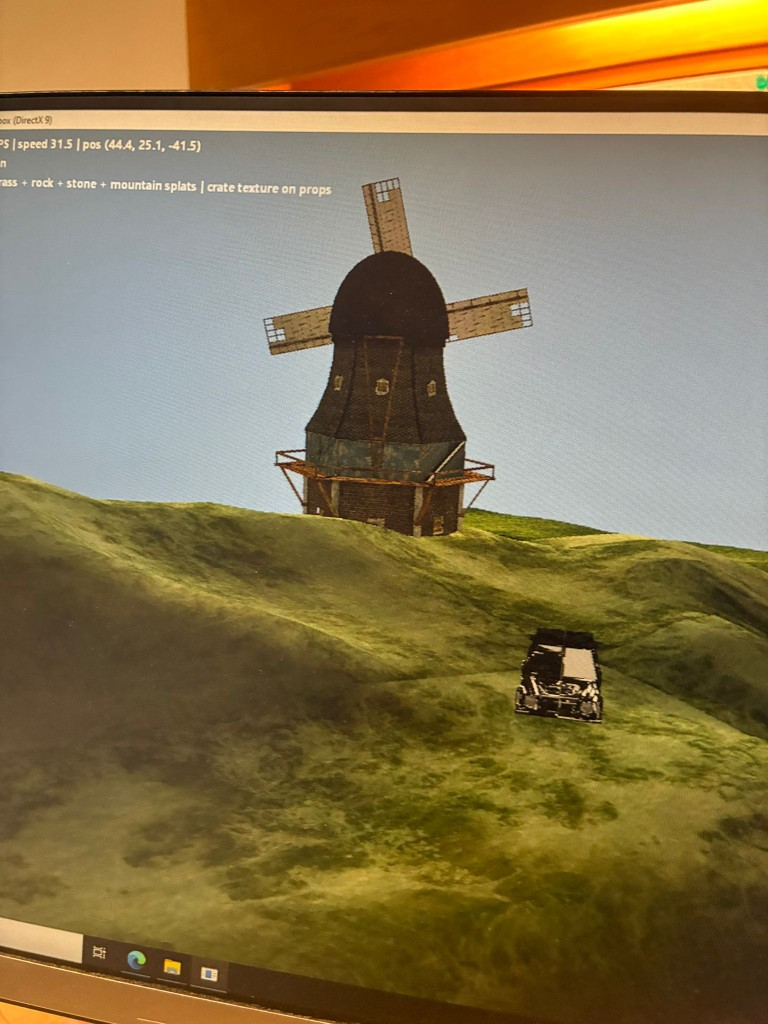
\includegraphics[trim=22 30 22 42,clip,width=0.92\linewidth]{screenshot_sandbox_windmill.png}}}
\newcommand{\ciScreenshot}{%
  \fcolorbox{AbstractFrame}{white}{%
    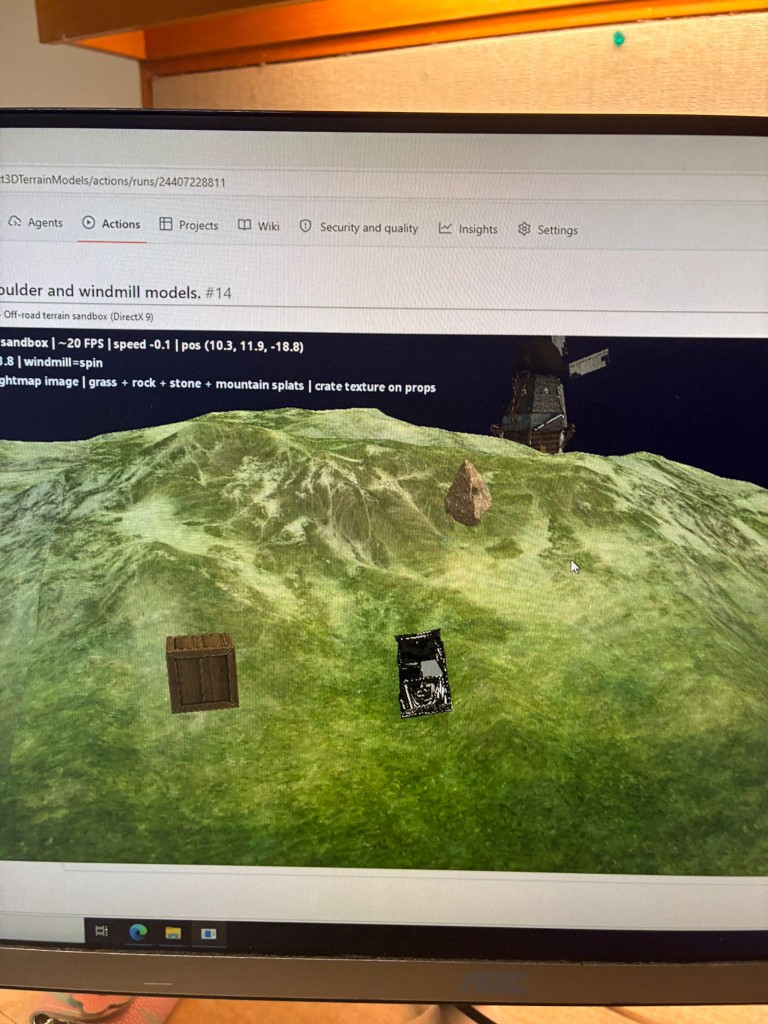
\includegraphics[trim=24 28 24 48,clip,width=0.92\linewidth]{screenshot_github_actions_run.png}}}

\begin{document}
\renewcommand{\figurename}{\textcolor{Brand}{Figure}}
\maketitle
\thispagestyle{empty}
\vspace*{-1.5em}

\begin{reportabstract}
This project is a DirectX~9.0c sandbox (not a scored game) where a player drives an off-road vehicle on procedural mountainous terrain. The build supports keyboard and XInput gamepad control, third-person chase camera, terrain splatting, collision with static and dynamic props, windmill animation, and a day/night lighting cycle. This report is intentionally concise: deliverables first, then implementation and authorship evidence.
\end{reportabstract}

\tableofcontents
\newpage

\section{Project snapshot}\sectionrule
\label{sec:snapshot}

\subsection{What is delivered}
\begin{itemize}
  \item Executable package: \texttt{Game\_Build/maeg4060\_stage2.exe} with \texttt{Game\_Build/Assets/}.
  \item Source code: \texttt{src/} and \texttt{CMakeLists.txt}.
  \item Documentation: Stage PDFs (\texttt{stageOne.pdf}, \texttt{stageTwo.pdf}, \texttt{stageFinal.pdf}) plus the \textbf{standalone user guide} \texttt{docs/User\_Guide.pdf} (controls, requirements, and troubleshooting; summarized in \S\ref{sec:run}).
  \item Public repository (for markers, version control, and CI):\newline
        {\small\url{https://github.com/Rex-Yim/Direct3DTerrainModels}}.
  \item Media: figures in this PDF; short viewport recordings under \texttt{docs/media/}; README GIFs under \texttt{docs/images/}.
\end{itemize}

\subsection{Course expectations mapping}
Table~\ref{tab:marking} maps typical final-stage submission themes from the course project brief to sections of this report, companion PDFs, and code entry points.

\begin{table}[htbp]
  \centering
  \small
  \setlength{\tabcolsep}{6pt}
  \begin{tabular}{@{}p{0.34\linewidth}p{0.58\linewidth}@{}}
    \toprule
    \textbf{Theme} & \textbf{Where it is covered} \\
    \midrule
    Input (keyboard / XInput) & \S\ref{sec:run}; implementation in \texttt{src/Input.cpp} \\
    Terrain height \& vehicle following & \S\ref{sec:terrain}; \texttt{src/Terrain.cpp}, \texttt{src/Vehicle.cpp} \\
    Collision \;\&\; physics-based motion & \S\ref{sec:physics}; \texttt{src/Collision.cpp}, \texttt{Vehicle.cpp}, boulder logic in \texttt{Game.cpp} \\
    Animation / hierarchy models & \S\ref{sec:animation}; \texttt{src/AnimatedModel.cpp}, windmill update/draw in \texttt{Game.cpp} \\
    Authorship \;\&\; media evidence & \S\ref{sec:assets}; assets under \texttt{Assets/models/} \\
    Build, D3DX, packaging & \S\ref{sec:build}; \texttt{CMakeLists.txt}, Appendix-style notes in \S\ref{sec:build} \\
    User guide (separate PDF) & \texttt{docs/User\_Guide.pdf} (full detail); \S\ref{sec:run} for a short extract \\
    \bottomrule
  \end{tabular}
  \caption{Index for marking: themes vs.\ sections and code.}
  \label{tab:marking}
\end{table}

\subsection{Core features}
\begin{itemize}
  \item Procedural heightfield terrain with bilinear height sampling.
  \item Grass base plus slope/height-driven splat layers (rock, stone, mountain).
  \item Vehicle driving with steering, throttle/brake, and terrain-normal alignment.
  \item Windmill: hierarchical \texttt{.x} with \texttt{ID3DXAnimationController} when keyframed data is present; static mesh path uses subset draws / code-driven motion when animation sets are absent (\S\ref{sec:animation}).
  \item Collision with crate (AABB) and dynamic boulder (sphere, gravity, impulse).
  \item HUD: smoothed FPS, speed, world position, simulation clock, windmill mode (animation vs.\ static spin vs.\ paused), terrain mode/splat summary, optional mini-map/legend; plus day/night lighting.
\end{itemize}

\subsection{Runtime screenshots}
\begin{figure}[htbp]
  \centering
  \sandboxScreenshot
  \caption{In-application view: procedural splats, windmill, vehicle, props, and HUD.}
  \label{fig:runtime}
\end{figure}

\begin{figure}[htbp]
  \centering
  \ciScreenshot
  \caption{GitHub Actions workflow run showing the integrated sandbox result.}
  \label{fig:ci}
\end{figure}

\section{How to run and evaluate}\sectionrule
\label{sec:run}

\subsection{System requirements}
Windows 10 or later (64-bit recommended), DirectX~9 compatible GPU, display at least $1280\times720$. Optional Xbox-compatible controller (XInput).

\subsection{Launch}
Run \texttt{maeg4060\_stage2.exe} from \texttt{Game\_Build} with \texttt{Assets} beside the executable. Build details are summarized in \S\ref{sec:build}. The \textbf{standalone user guide} deliverable (\texttt{docs/User\_Guide.pdf}) contains the authoritative control list, requirements, and troubleshooting; this section duplicates only the essentials.

\subsection{Controls}
\begin{center}
\renewcommand{\arraystretch}{1.18}
\begin{tabular}{@{}>{\bfseries}p{3.15cm}p{6.85cm}@{}}
  \toprule
  \multicolumn{1}{@{}l}{\textcolor{Brand}{\textbf{Input}}} &
  \multicolumn{1}{l}{\textcolor{Brand}{\textbf{Action}}} \\
  \midrule
  W / S & Throttle forward / reverse \\
  A / D & Steer left / right \\
  Space & Brake \\
  M & Pause / resume windmill animation \\
  Esc & Exit application \\
  \bottomrule
\end{tabular}
\end{center}

\medskip
\noindent\textbf{Gamepad:} left stick steers; right trigger throttles; left trigger brakes / partial reverse.

\subsection{Quick troubleshooting}
\begingroup\sloppy
\begin{itemize}
  \item Missing D3DX DLL: install the legacy DirectX end-user runtime, or ship \texttt{D3DX9\_43.dll} next to the exe when the build copies it.
  \item Missing models or textures: keep \texttt{Assets/} next to the executable (working directory must resolve relative paths).
  \item Blank screen after window resize: the sample calls font and device lost/reset around \texttt{IDirect3DDevice9::Reset}---confirm GPU drivers; see user guide if issues persist.
\end{itemize}
\endgroup

\section{Implementation summary}\sectionrule
\label{sec:impl}

\subsection{Frame pipeline}
The loop is input $\rightarrow$ update $\rightarrow$ render. Input uses \texttt{GetAsyncKeyState} and \texttt{XInput\-Get\-State}; update integrates vehicle and boulder motion, resolves collisions, advances animation timing, and updates lighting; render draws terrain, models, and HUD via the fixed-function Direct3D~9 pipeline.

\subsection{Terrain and navigation}
\label{sec:terrain}
Terrain height uses bilinear interpolation:
\[
h(x,z) = (1-t_x)(1-t_z)h_{00} + t_x(1-t_z)h_{10} + (1-t_x)t_z h_{01} + t_x t_z h_{11}.
\]
The vehicle aligns its up vector with the local terrain normal; steering sets yaw for stable hill following.

\subsection{Physics and collision}
\label{sec:physics}
Crate: AABB tests. Boulder: bounding sphere with gravity and simple impulses on vehicle contact (lightweight dynamic object).

\subsection{Animation and rendering}
\label{sec:animation}
\textbf{Windmill.}\quad
If the hierarchy load from \texttt{model\_windmill.x} succeeds and reports animation sets, \texttt{Game::Update} advances \texttt{ID3DXAnimationController} time each frame (unless paused with \texttt{M}). If loading falls back to static geometry (OBJ or static \texttt{.x}), the renderer uses mesh subset draws; sail motion may be driven in code for that path---not via the keyframed controller.

\medskip
\noindent\textbf{Scene lighting.}\quad
A day/night style effect moves the sun direction and interpolates clear and ambient colours (\texttt{Game.cpp}).

\section{3D models, media, and authorship}\sectionrule
\label{sec:assets}

\subsection{Authorship statement}
Vehicle, windmill, crate, and boulder meshes/materials under \texttt{Assets/models/} are original work by Guo Tsun Hei. Runtime terrain is generated procedurally. Sketchfab links in Stage~1 were references only, not shipped geometry.

\subsection{Integration notes}
\begingroup\sloppy
\noindent\textbf{Jeep, crate, and boulder.}\quad
\texttt{Game::Initialize} calls \texttt{LoadStaticModelCandidates} in \texttt{src/Game.cpp}; each candidate path is tried until one loads.

\begin{itemize}\setlength\itemsep{0.25em}
  \item \textbf{Jeep:} four attempts (bundled OBJ, flat replacement OBJ, root \texttt{model\_jeep.obj}, then \texttt{model\_jeep.x}).
  \item \textbf{Crate / boulder:} three OBJ attempts each (bundled, flat replacement, then root models folder). No \texttt{.x} list; if all fail, a textured box or sphere is built.
\end{itemize}

\noindent\textbf{Windmill.}\quad
The animated hierarchy at \texttt{Assets/models/model\_windmill.x} is tried first. If that fails, static OBJs are tried in the same folder pattern as other props, with \texttt{model\_windmill.x} last (no animation).

\medskip
\noindent\textbf{Scene setup.}\quad
After load, meshes are placed in world space; \texttt{BuildReplacementMeshCorrection} adjusts orientation and scale where needed.
\endgroup

\subsection{Static figure evidence}

\subsubsection{Authoring-tool viewports}
These stills support texture work and scale; playable terrain remains procedural (see \texttt{Terrain.cpp}).

\begin{figure}[htbp]
  \centering
  \setlength{\fboxsep}{5pt}%
  \setlength{\fboxrule}{0.55pt}%
  \fcolorbox{AbstractFrame}{white}{%
    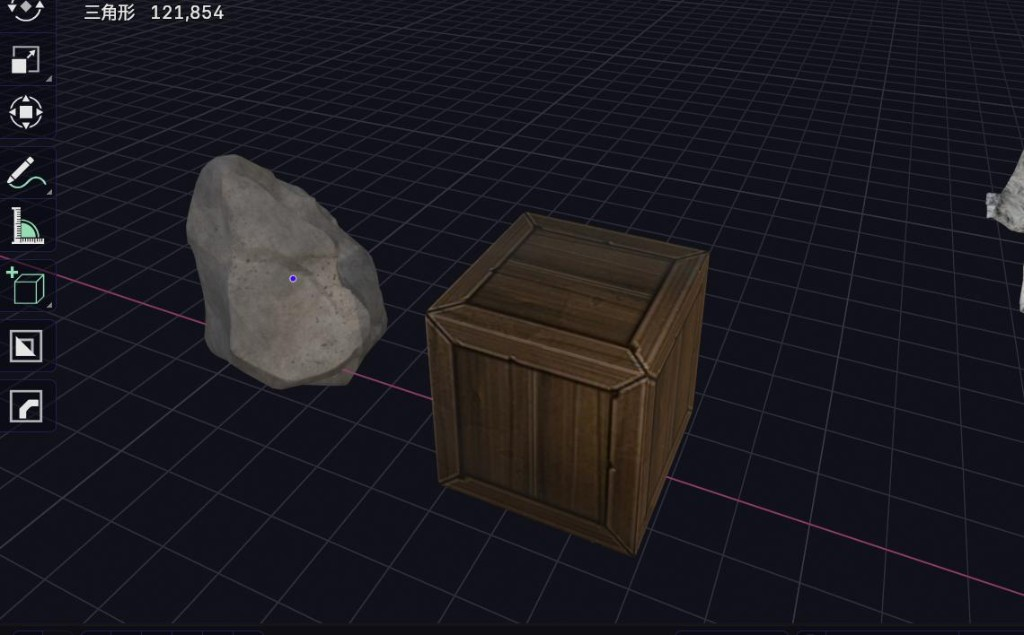
\includegraphics[width=\AuthfigWidth]{modeling_viewport_crate_boulder.png}}
  \caption{Crate and boulder meshes in the authoring viewport.}
  \label{fig:modeling-crate}
\end{figure}

\begin{figure}[htbp]
  \centering
  \setlength{\fboxsep}{5pt}%
  \setlength{\fboxrule}{0.55pt}%
  \fcolorbox{AbstractFrame}{white}{%
    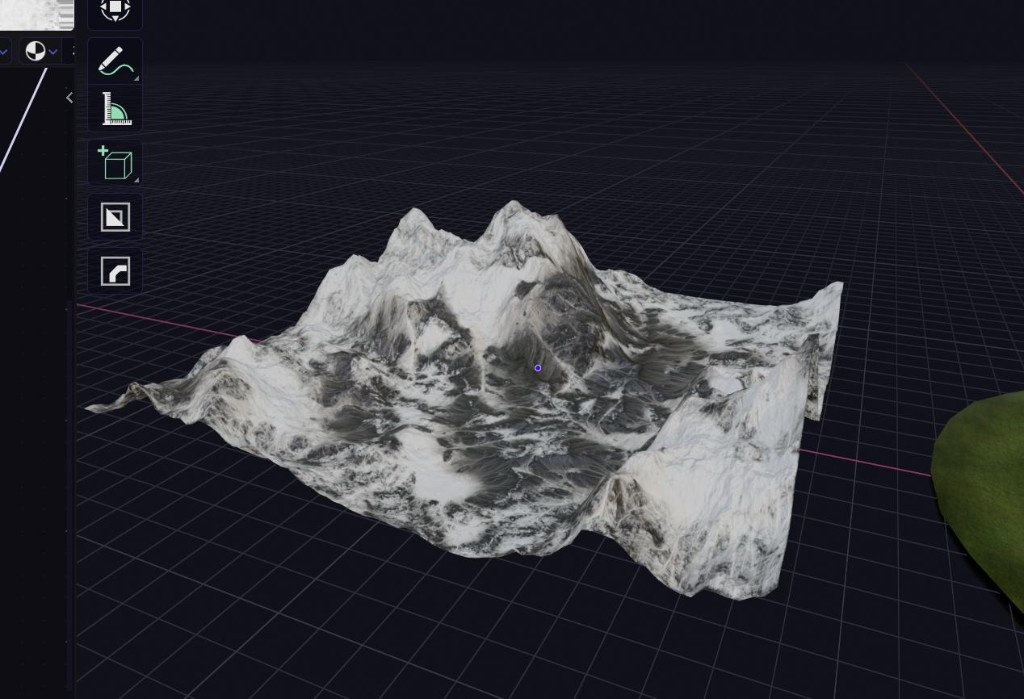
\includegraphics[width=\AuthfigWidth]{modeling_viewport_terrain.png}}
  \caption{Terrain sculpt and materials in the authoring tool (\emph{playable hills are procedural in the exe}).}
  \label{fig:modeling-terrain}
\end{figure}

\subsubsection{Cinema 4D source frames (jeep and windmill)}
Representative frames from screen recordings under \texttt{docs/media/}; GIF variants are listed in \S\ref{sec:video-readme}.

\begin{figure}[htbp]
  \centering
  \setlength{\fboxsep}{5pt}%
  \setlength{\fboxrule}{0.55pt}%
  \fcolorbox{AbstractFrame}{white}{%
    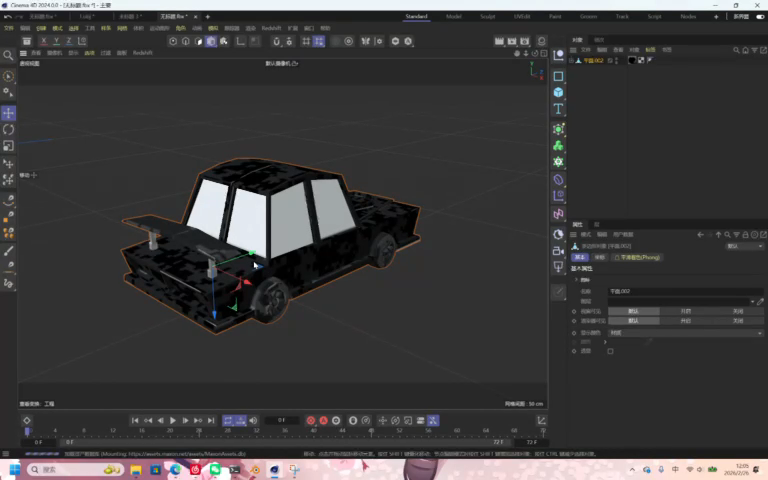
\includegraphics[width=\AuthfigWidth]{c4d_car_viewport_frame.png}}
  \caption{Jeep source model: Cinema~4D viewport (frame from recorded session).}
  \label{fig:c4d-jeep}
\end{figure}

\begin{figure}[htbp]
  \centering
  \setlength{\fboxsep}{5pt}%
  \setlength{\fboxrule}{0.55pt}%
  \fcolorbox{AbstractFrame}{white}{%
    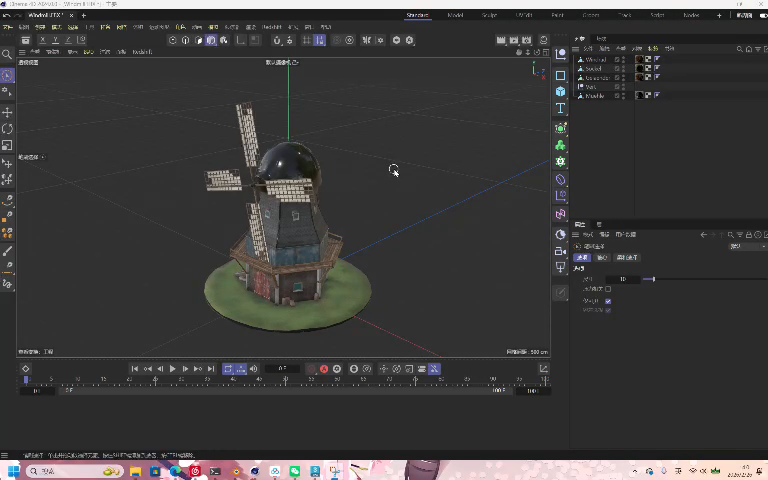
\includegraphics[width=\AuthfigWidth]{c4d_windmill_viewport_frame.png}}
  \caption{Windmill source model: Cinema~4D viewport (frame from recorded session).}
  \label{fig:c4d-windmill}
\end{figure}

\subsection{Video and README media}
\label{sec:video-readme}
\noindent Recordings (paths in repo):\quad \texttt{docs/media/c4d-car-viewport.mp4} and\\
\texttt{docs/media/c4d-windmill-viewport.mp4}.\\
GIFs for the GitHub README live under \texttt{docs/images/}.

\section{Build and packaging notes}\sectionrule
\label{sec:build}

\subsection{Toolchain}
Windows CMake, C++17, MSVC recommended. Target \texttt{maeg4060\_stage2}. Links \texttt{d3d9}, \texttt{d3dx9}, \texttt{xinput9\_1\_0}.

\subsection{D3DX path}
\begingroup\sloppy\small
\noindent\textbf{(1)}~Set \texttt{DXSDK\_DIR} to the June 2010 DirectX SDK.\quad
\textbf{(2)}~Or configure without it and let CMake obtain the NuGet D3DX package (see \texttt{CMakeLists.txt}).\par
\noindent Post-build or install steps may copy \texttt{D3DX9\_43.dll} beside the executable when available.
\endgroup

\subsection{Packaging target}
Submit the full \texttt{Game\_Build} folder (executable, \texttt{Assets/}, required DLLs), not the \texttt{.exe} alone.

\section{Conclusion}\sectionrule
\label{sec:conclusion}
The deliverable is a compact DirectX~9 sandbox: terrain navigation, input, collision, animation integration, and team-authored 3D content. Submission materials include this report, the standalone user guide PDF, staged course PDFs, source, \texttt{Assets/}, and build instructions; the public GitHub repository hosts the CI-backed tree used for integration screenshots.

\medskip
\noindent\textbf{Known limitations.}\quad
There is no audio engine. The jeep has no per-wheel articulation in code. Terrain is procedural at runtime rather than a single imported artist heightmap (optional image heightfields are supported when assets exist). The boulder uses simplified sphere--box response rather than full rigid-body stacks. These bounds keep the codebase small while meeting sandbox and course demonstration goals.

\medskip
\noindent\textbf{Possible extensions.}\quad
Import a large heightmap PNG, extend rigging for wheel bones, add richer rigid-body contact, and optional PBR or shader-based terrain beyond the fixed-function pipeline.

\section{References}\sectionrule
\begingroup\sloppy\small
\begin{itemize}
  \item MAEG4060 Virtual Reality Systems and Applications --- course project description (2025--26, Semester~2), CUHK Faculty of Engineering.
  \item Microsoft Learn / MSDN: Direct3D~9, D3DX~9 utilities, XInput.\newline
        \url{https://learn.microsoft.com/en-us/windows/win32/direct3d9}
  \item D3DX via NuGet package \texttt{Microsoft.DXSDK.D3DX}; see \texttt{CMakeLists.txt}.
  \item CMake documentation: \url{https://cmake.org/documentation/}
  \item GitHub repository and CI:\newline
        \url{https://github.com/Rex-Yim/Direct3DTerrainModels}
  \item Local checkout: \texttt{src/}, \texttt{CMakeLists.txt}, \texttt{docs/User\_Guide.pdf}.
\end{itemize}
\endgroup

\end{document}
